\chapter{Benchmark Datasets}
\label{chap:datasets}

In this chapter, we detail the datasets used to evaluate and compare the performance of the A* training framework against standard Stochastic Gradient Descent (SGD). To provide a comprehensive assessment, the benchmarks cover both regression and classification tasks, ranging from synthetic functional mappings to high-dimensional real-world data. 

For all experiments, a uniform data partitioning strategy was applied, splitting each dataset into training, validation, and test sets according to an 80-10-10 percentage ratio.

\section{Regression Datasets}

\subsection{Noisy Sine Function}
\label{sec:ds_sine}
The Noisy Sine dataset is a synthetic benchmark designed to assess the algorithm's ability to capture non-linear, periodic patterns in a low-dimensional setting. The dataset consists of 1,000 samples generated from a one-dimensional sine wave.

\begin{itemize}
    \item \textbf{Data Generation:} The samples are evenly spaced in the range $x \in [0, 4\pi]$.
    \item \textbf{Noise Profile:} To simulate real-world variance, additive Gaussian noise was introduced: $y = \sin(x) + \epsilon$, where $\epsilon \sim \mathcal{N}(0, 0.1)$.
\end{itemize}

\begin{center}
\begin{figure}[H]
    \centering
    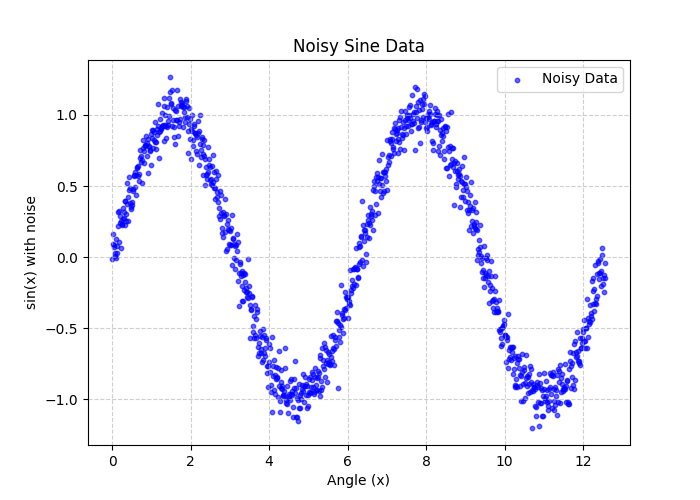
\includegraphics[width=0.8\textwidth]{figures/sine_tests/sine_dataset.png}
     \caption{Plot of the noisy sine dataset}
\end{figure}
\end{center}


\subsection{California Housing}
\label{sec:ds_california}
The California Housing dataset provides a high-dimensional, real-world regression challenge. Derived from the 1990 U.S. Census, it contains 20,640 samples, each representing a specific California district.

\begin{itemize}
    \item \textbf{Input Features:} 8 economic and geographic features, including Median Income (MedInc), House Age, Average Rooms, and spatial coordinates (Latitude/Longitude).
    \item \textbf{Target:} The median house value for the district, expressed in units of \$100,000.
\end{itemize}

\section{Classification Datasets}

\subsection{Iris Flower}
\label{sec:ds_iris}
The Iris dataset is a classic multiclass classification benchmark. It is a relatively small but well-structured dataset consisting of 150 samples distributed equally across three species of Iris flowers.

\begin{itemize}
    \item \textbf{Input Features:} 4 physical measurements (sepal length, sepal width, petal length, and petal width).
    \item \textbf{Class Distribution:} Three species: \textit{Setosa}, \textit{Versicolor}, and \textit{Virginica}.
\end{itemize}



\subsection{Wine Quality (Red)}
\label{sec:ds_wine}
The Wine Quality dataset offers a more complex classification task due to its higher dimensionality and larger sample size (1,599 samples) compared to the Iris dataset. It captures the physicochemical properties of Portuguese "Vinho Verde" red wine.

\begin{itemize}
    \item \textbf{Input Features:} 11 physicochemical variables, including fixed acidity, volatile acidity, residual sugar, chlorides, pH, sulphates, and alcohol content.
    \item \textbf{Class Distribution:} The original dataset contains quality scores ranging from 3 to 8. These are shifted to a 0--5 range for modeling.
\end{itemize}

\section{Summary of Dataset Characteristics}

The table below summarizes the dimensions and objectives of the employed benchmarks.

\begin{table}[htbp]
\centering
\caption{Summary of Benchmark Datasets}
\label{tab:dataset_summary}
\begin{tabular}{lcccc}
\hline
\textbf{Dataset} & \textbf{Type} & \textbf{Samples} & \textbf{Features} & \textbf{Output Classes} \\ \hline
Noisy Sine & Regression & 1,000 & 1 & N/A \\
California Housing & Regression & 20,640 & 8 & N/A \\
Iris Flower & Classification & 150 & 4 & 3 \\
Wine Quality & Classification & 1,599 & 11 & 6 \\ \hline
\end{tabular}
\end{table}